\label{sec:phase}

The corrected first-order condition from \Cref{sec:mixing} is one algebraic equation, but its solution can fall in different parts of the feasible interval $[0,n]$. Which case occurs depends on two exponents: the generator bias-decay exponent $\beta$ and the synthetic-variance exponent $\rho$ from Assumption~\ref{asm:pl} and~\ref{asm:vn}. This section maps those cases. \Cref{ssec:critical} studies the shape of the risk curve, \Cref{ssec:phase} states the five-regime phase diagram, and \Cref{ssec:risk} gives the risk rates; \Cref{app:plateau} explains what changes when the generator has irreducible bias.

\subsection{Critical-point structure}\label{ssec:critical}

Multiplying both sides of the first-order condition \cref{eq:foc} by $x^{2\beta+1}$ removes negative powers of $x$ and leaves one object to study:
\begin{equation}\label{eq:Phi-def}
  \Phi(x)\;:=\;\bigl(v_n+cx^{-2\beta}\bigr)^2 x^{2\beta+1}\;=\;B_n(x)^2\,x^{2\beta+1},
\end{equation}
The function $\Phi$ is monotone when learning is slow and U-shaped when learning is fast. Critical points of $R_n(x)$ are exactly the roots of $\Phi(x)=2\beta a c$. Thus the number of candidate optima is determined by the shape of this one curve.

\begin{lemma}[Critical points of $R_n$]\label{lem:critical}
Assume Assumption~\ref{asm:pl} and~\ref{asm:vn} with $a, c, v_n>0$.
\begin{enumerate}[label=\rm(\roman*),leftmargin=*]
\item If $\beta\le 1/2$, then $\Phi$ is strictly increasing on $(0,\infty)$, so $R_n$ has at most one interior critical point on $(0,n)$, and when it exists it is a strict local minimum. For $\beta<1/2$ the critical point exists for every $v_n>0$; for $\beta=1/2$ it exists if and only if $a>c$.
\item If $\beta>1/2$, then $\Phi$ is strictly U-shaped with unique minimum at
  \begin{equation}\label{eq:xdagger}
    x^\dagger\;=\;\biggl(\frac{c\,(2\beta-1)}{(2\beta+1)\,v_n}\biggr)^{1/(2\beta)},\qquad \Phi^\dagger\;:=\;\Phi(x^\dagger)\;\propto\;c^{(2\beta+1)/(2\beta)}\,v_n^{(2\beta-1)/(2\beta)}.
  \end{equation}
When $\Phi^\dagger<2\beta a c$, $R_n$ has exactly two interior critical points $x_1<x^\dagger<x_2$; the smaller is a local maximum and the larger, $x_n^\circ:=x_2$, is the unique interior local minimum. When $\Phi^\dagger\ge 2\beta a c$, $R_n$ has no interior local minimum. Under Assumption~\ref{asm:vn} with $\rho>0$, $\Phi^\dagger\to 0$, so the two-root regime holds for all sufficiently large $n$.
\end{enumerate}
\end{lemma}

That is to say, when the generator learns slowly ($\beta\le 1/2$), the bias term $cx^{-2\beta}$ decays gently and the profiled risk has at most one interior minimum. When the generator learns quickly ($\beta>1/2$), the bias decays steeply enough that $\Phi$ first falls and then rises. The active minimum is the larger of the two roots; the smaller root is a local maximum and is not useful for allocation. The value $\Phi^\dagger$ tells us whether the dip falls below $2\beta a c$. Once $n$ is large enough, it does, so the active root $x_n^\circ$ exists.

\subsection{Phase diagram}\label{ssec:phase}

The asymptotic location of the active root $x_n^\circ$, and hence of the global oracle $x_n^\star\in\argmin_{x\in[0,n]}R_n(x)$, depends on $(\beta,\rho)$ in five distinct ways.

\begin{theorem}[Allocation phase diagram]\label{thm:phase}
Assume Assumption~\ref{asm:pl} and~\ref{asm:vn}. Let $x_n^\circ$ denote the active interior root from \Cref{lem:critical} (when it exists) and $x_n^\star\in\argmin_{x\in[0,n]}R_n(x)$ the global oracle. As $n\to\infty$:

\smallskip
\noindent\textbf{Regime~I (persistent synthetic variance, $\rho=0$).} Every interior critical point is $O(1)$, so $\lambda_n^\star=x_n^\star/n\to 0$ regardless of $\beta$.

\smallskip
\noindent\textbf{Regime~II (slow learning, $\beta<1/2$, $\rho>0$).} $x_n^\circ\to x_\infty:=(2\beta a/c)^{1/(1-2\beta)}\in(0,\infty)$, hence $x_n^\circ=O(1)$ and $\lambda_n^\star\to 0$. The first-order rate of $R_n(x_n^\star)$ matches the all-real rate $a/n$, with strict finite-sample shrinkage.

\smallskip
\noindent\textbf{Regime~III (sublinear calibration, $\beta>1/2$, $0<\rho<\beta+\tfrac12$).} For all sufficiently large $n$, the active interior root exists and satisfies
\begin{equation}\label{eq:xn-circ-III}
  x_n^\circ\;=\;\Bigl(\tfrac{2\beta ac}{v_0^2}\Bigr)^{1/(2\beta+1)}\,n^{2\rho/(2\beta+1)}\,\bigl\{1+o(1)\bigr\}.
\end{equation}
Consequently $\lambda_n^\circ=x_n^\circ/n\asymp n^{2\rho/(2\beta+1)-1}\to 0$, and the safe-improvement condition of \Cref{prop:safe} holds asymptotically: $x_n^\circ\,B_n(x_n^\circ)\to 0<a$. Hence $x_n^\star=x_n^\circ\{1+o(1)\}$.

\smallskip
\noindent\textbf{Regime~IV (full calibration, $\beta>1/2$, $\rho>\beta+\tfrac12$).} The unconstrained Regime~III root would exceed the real-data budget: $x_n^\circ\gg n$. The constrained oracle therefore pins to the boundary $x=n$, where $B_n(n)=v_n+cn^{-2\beta}=o(n^{-1})$. Thus $\lambda_n^\star\to 1$ and $R_n(x_n^\star)=v_n+cn^{-2\beta}=o(n^{-1})$, beating the all-real rate.

\smallskip
\noindent\textbf{Regime~V (parametric knife-edge, $\beta=1/2$).} An interior root exists iff $a>c$; in that case $x_n^\circ=(\sqrt{ac}-c)\,n^\rho/v_0\,\{1+o(1)\}$. The boundary regime depends on $\rho$ and on the constants $(a,c,v_0)$: for $\rho<1$, $\lambda_n^\circ\to 0$ with $R_n(x_n^\star)=a/n\{1+o(1)\}$ and a strict finite-sample improvement; for $\rho=1$, $\lambda_n^\circ\to(\sqrt{ac}-c)/v_0\in(0,1)$ provided $\sqrt{ac}-c<v_0$; for $\rho>1$, $\lambda_n^\star\to 1$ if $c<a$. If $a\le c$, no interior root exists and $x_n^\star=0$.
\end{theorem}

\Cref{fig:phase} shades the $(\beta,\rho)$ plane by these five regimes. The main case is the row $\rho=1$, $\beta>1/2$ inside Regime~III. When synthetic and real budgets scale together and the generator learns faster than parametric, \cref{eq:xn-circ-III} gives $x_n^\star\asymp n^{2/(2\beta+1)}$. The optimal calibration size grows, but sublinearly, so the calibration share $\lambda_n^\star\to 0$. This explains why positive fixed-share baselines, including $\lambda=2\beta/(1+2\beta)$, over-calibrate in the common regime $m_n\asymp n$.

\subsection{Risk consequences}\label{ssec:risk}

Inside Regime~III the variance side $V_R(x_n^\circ)\sim a/n$ and bias side $B_n(x_n^\circ)\sim v_n$ collapse the harmonic-mean profiled risk into one of three subcases driven by whether the synthetic budget grows slower than, in step with, or faster than the real budget:
\begin{equation}\label{eq:Rn-III}
  R_n(x_n^\star)\;=\;\frac{V_R(x_n^\circ)\,v_n}{V_R(x_n^\circ)+v_n}\,\bigl\{1+o(1)\bigr\}\;=\;\begin{cases}\dfrac{a}{n}\{1+o(1)\}&\text{if }\rho<1,\\[6pt]\dfrac{a v_0}{(a+v_0)\,n}\{1+o(1)\}&\text{if }\rho=1,\\[6pt]\dfrac{v_0}{n^\rho}\{1+o(1)\}&\text{if }\rho>1.\end{cases}
\end{equation}
The three branches have a simple interpretation. If $\rho<1$, synthetic sampling noise is too large to change the first-order rate, so the risk matches all-real up to a smaller-order gain. If $\rho=1$, real and synthetic variances are both order $1/n$, and pooling gives a strictly smaller leading constant than $a/n$. If $\rho>1$, the synthetic side is accurate enough that the risk is faster than $1/n$, so all-real estimation is first-order suboptimal.

% [Subsection ``Plateau bias'' moved to Appendix~\ref{app:plateau} to fit
%  the 9-page main-content limit; statement and discussion are reproduced
%  there verbatim, and \Cref{prop:plateau} is still proved in
%  \Cref{proof:plateau}.]


\begin{figure}[!t]
  \centering
  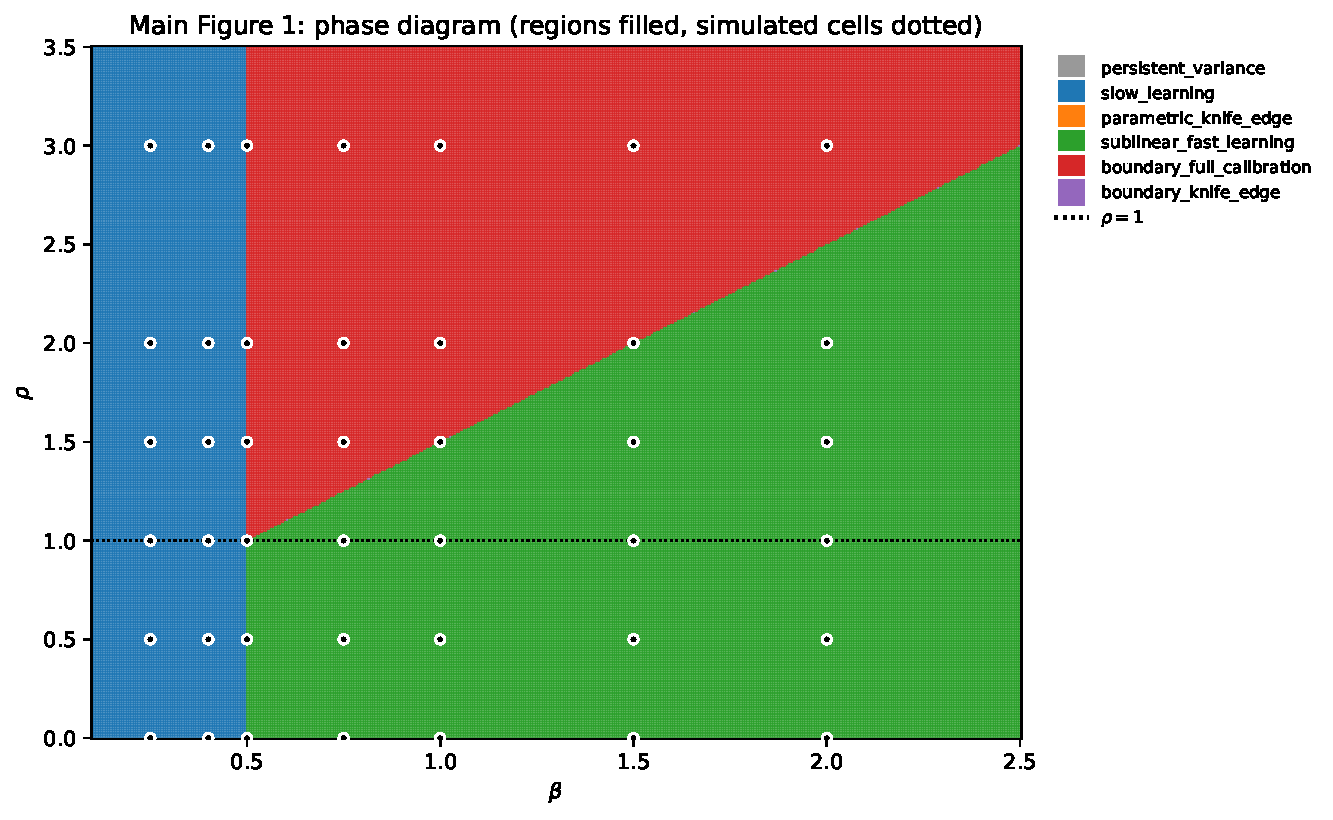
\includegraphics[width=0.7\linewidth]{figures/fig1_phase_diagram.pdf}
  \caption{Theoretical phase diagram in $(\beta,\rho)$ space. The five regimes of Theorem~\ref{thm:phase} partition the plane by the asymptotic behavior of the optimal calibration size $x_n^\star$. The horizontal line $\rho=1$ is the empirically common case in which the synthetic budget scales linearly with the real budget; the vertical line $\beta=1/2$ is the parametric knife edge. The labelled headline regime is the wide wedge $\beta>1/2$, $0<\rho<\beta+\tfrac12$, where the optimal calibration share vanishes despite the optimal calibration size diverging.}
  \label{fig:phase}
\end{figure}

% POLISHED
